\chapter{State of Science and Technology}%
\label{chap:StateOfArt}%

Autonomous and automated vehicles must have a comprehesive and accurate understanding of their surroundings at 
all times to ensure safe and reliable operation. This process, known as environment perception, is responsible
for detecting, identifying, and tracking objects such as other vehicles, cyclists, pedestrians or other
road elements. The quality of the measurement of the state of this objects directly influence the vehicle's
ability to make safe and informed driving decisions. 

Failures in the perception can lead to hazarous situations, such as collisions or unexpected navigation decisions.
This is particularly critical in high-speed scenarios or complex urban environments, where is a high density of
high dynamic objects which make more complex the operation in real time. 

A robust perception system must provide the following capabilities:

\begin{enumerate}
  \item \textbf{Object detection:} Identify and locate objects in the vehicle's surroundings, such as vehicles, pedestrians, cyclists, or other road elements.
  \item \textbf{Motion estimation:} Determining the position and velocity of moving objects
  \item \textbf{Scene understanding:} Classifiying the detected objects and assessing their criticality for the vehicle's navigation
  \item \textbf{Reliability in edge cases:} Ensuring correct operation in complex and unforeseen scenarios, such as occlusions, adverse weather conditions, or sensor failures.
  \item \textbf{Real-time operation:} Providing timely and accurate information to the vehicle's control system to make informed driving decisions.
\end{enumerate}

While the perception concept includes different aspects, this work will focus specifically on the detection of 
moving object in the vehicle's surroundings and the estimation of their 6D motion state (position and velocity) 
using a deterministic approach. In the following sections, we will provide an overview of the state-of-the-art of
the different sensors and algorithms used in the perception systems of autonomous vehicles, focusing on the deterministic image
based approaches.

\subsection{Perception Techniques in Autonomous Vehicles}

The perception systems of autonomous vehicles rely on a combination of different sensors to provide a 
comprehensive understanding of the ego vehicle's surroundings. In this section we will provide an overview of
the most common sensor types used in autonomous vehicles and their advantages and limitations.

\subsubsection{LiDAR-Based Perception}

LiDAR (Light Detection and Ranging) sensors are increasingly used in the automotive industry for 
obstacle detection, 3D mapping and lane detection \cite{autonomous_vehicles_perception_survey}. More and more companies are adopting this type of sensor due to its advantage 
in rapidly and accurately estimating 3D distances. Examples include BMW~\cite{lidarbased_bmw}, 
Merceces-Benz~\cite{lidarbased_mercedes}, and Waymo~\cite{lidarbased_waymo}.

\paragraph{Working principle}

LiDAR sensors use the concept of time of flight to measure the distance to objects in the vehicle's surroundings.
The sensor emits a laser beam and measures the time it takes for the light to reflect back to the sensor.
By calculating the time difference, the sensor can determine the distance to the object based 
on the speed of light \cite{lidarbased_review}.

\paragraph{Advantages and Limitations}

LiDAR sensors have the advantage of providing an accurate 3D representation of the vehicle's surroundings.
This makes them particularly useful for object detection and localization tasks. However, LiDAR sensors
are sensitive to adverse weather conditions, such as rain, snow or fog since the laser beams can be scattered
by the particles in the air. Additionally, LiDAR sensors are more expensive than other sensor types, such as
cameras or radars, which can limit their adoption in mass-market vehicles, although their prices are steadily decreasing \cite{autonomous_vehicles_perception_survey}.

\subsubsection{Radar-Based Perception}

Radar (Radio Detection and Ranging) use radio waves to detect objects in the vehicle's surroundings. They are commonly
used in the automotive industry for object avoidance. 

\paragraph{Working principle} Similar to LiDAR sensors, radar sensors emit radio waves and measure the time it takes for the waves to reflect back to the sensor. 
By calculating the time difference, the sensor can determine the distance to the object based on the speed of light. 
Radar sensors can also estimate the object's velocity based on the Doppler effect \cite{radarbased_velocity}.

\paragraph{Advantages and Limitations} Radar sensors are less sensitive to adverse weather conditions than LiDAR sensors, making them more reliable in rain, snow, or fog. \cite{autonomous_vehicles_perception_survey, radarbased_weather}. 
However, radar sensors have a lower resolution than LiDAR sensors, which can limit their ability to detect small objects or provide detailed information about the object's shape.

\subsubsection{Image-Based Perception}

Image based perception systems use cameras to capture images of the vehicle's surroundings and are the principal sensor
in some companies like Tesla~\cite{tesla_autopilot}. These sensors can be used as single cameras for object detection
and classification  or in pairs to provide stereo vision, which allows for depth estimation and 3D reconstruction of the scene.
These type of sensors can also be used for optical flow computation and the ego motion estimation through visual odometry

\paragraph{Monocular vision} Monocular vision systems use a single camera to capture images of the vehicle's surroundings. 
These systems are commonly used for object detection and classification tasks, such as detecting pedestrians, cyclists, or other vehicles \cite{autonomous_vehicles_perception_survey}. 
Monocular vision systems are less expensive than stereo vision systems and can be easily integrated into existing vehicles. 
However, they have limitations in depth perception and 3D reconstruction, which can make it 
challenging to estimate the distance to objects accurately. 

\paragraph{Stereo vision} Stereo vision systems use two cameras to capture images of the vehicle's surroundings and
use the pinhole camera model \cite{pin_hole_camera_model} to estimate the depth of objects in the scene. By comparing the images from the two cameras,
the system can calculate the disparity between corresponding points in the images and use this information to estimate the
distance to the objects.
\paragraph{Advantages and Limitations} Image-based perception systems have the advantage of providing a rich and 
detailed information about the environment. Cameras can capture color information,
texture, and shape of objects, which can be useful for object detection and classification tasks. In addition, cameras are less
expensive than LiDAR sensors and can be easily integrated into existing vehicles. However, image-based perception systems are
sensitive to adverse weather conditions, such as rain, snow, or fog, which can affect the quality of the images and limit the system's performance. 
The algorithms used for object detection and tracking in image-based perception systems can also be computationally intensive, which can
affect the system's real-time performance.  

In the following table a summary of the advantages and limitations of the different sensor types used in autonomous vehicles is provided:

\begin{table}[htb]
  \begin{tabular}{|l|l|l|}
  \cline{1-3}
    Sensor type & Advantages & Limitations \\ \cline{1-3} 
    LiDAR & \begin{tabular}[c]{@{}l@{}}Accurate 3D representation\end{tabular} & \begin{tabular}[c]{@{}l@{}}Expensive and sensitive \\ to adverse weather conditions\end{tabular} \\ \cline{1-3} 
    Radar & Works in bad weather, detects velocity & Low spatial resolution \\ \cline{1-3} 
    Cameras & \begin{tabular}[c]{@{}l@{}}Rich scene details, color information, \\ Cheaper than the other considered sensors\end{tabular} & \begin{tabular}[c]{@{}l@{}}Depth perception is limited, affected by lighting,\\ expensive computation cost\end{tabular} \\ \cline{1-3} 

  \end{tabular}
  \caption{Summary of sensor types used in autonomous vehicles}
\label{tab:sensor_summary}
\end{table}

While sensors provide raw data about the environment, perception algorithms are responsible for interpreting 
this information to detect and track moving objects. These algorithms can be broadly classified into 
learning-based and deterministic approaches, as discussed in the following sections.

\subsection{Algorithms for Moving Object Detection}

The perception algorithms can also be classified into two main categories: learning-based and deterministic approaches.
Learning-based approaches use machine learning techniques, such as deep learning, and are data driven. In the other side, deterministic
approaches use mathematical models to estimate the state of the objects in the scene. In the following sections we will provide an overview
of the most common algorithms used for moving object detection in autonomous vehicles.

\subsubsection{Learning-Based Approaches}

Learning-based approaches have gained popularity in recent years. These 
methods use convolutional neural networks (CNNs), recurrent neural networks (RNNs), and transformers
to process the data coming from cameras, LiDARs, and radar systems. In the work done by Wen and Jo \cite{learning_based_perception_survey}, 
they provide a comprehensive review of the different learning-based approaches used in autonomous vehicles, which can be summarized in the 
following figure: 

\begin{figure}[!h]%
  \centering%

  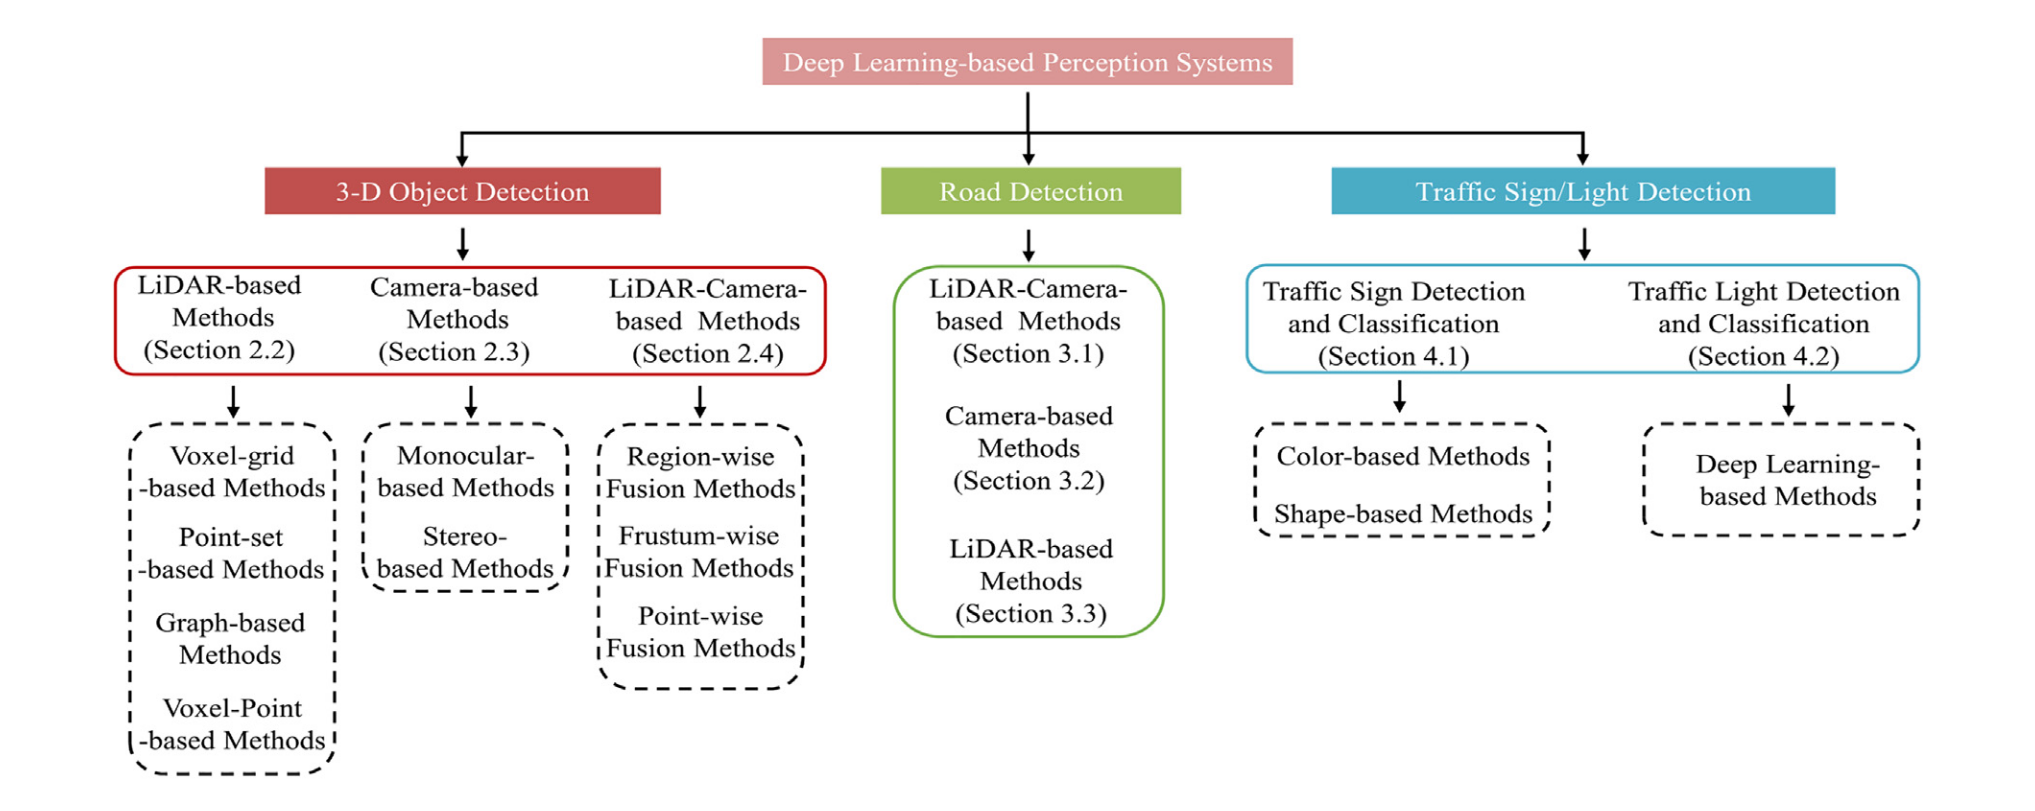
\includegraphics[width=135mm]{figures/learning_based_methods.png}%
  
  \caption{Learning-based perception methods. Source: \cite{learning_based_perception_survey}}%
  \label{fig:learning_based_methods}%
\end{figure}%

Some limitations of learning-based approaches are the need for extensive training data, which can be expensive and time-consuming to collect.
These methods can also struggle to generalize in novel and untrained scenarios, which can be problematic in safety-critical situations where the 
vehicle must make quick decisions based on the perceived environment.

\subsubsection{Deterministic Approaches}

Deterministic approaches use mathematical models to estimate the state of the objects in the scene. 

\paragraph{Optical flow}

Optical flow is a technique used to estimate the motion of objects in the scene by tracking the movement of pixels between consecutive frames.
This method is based on the assumption that the intensity of a pixel remains constant over time, which allows the system to track the movement
of objects based on the changes in pixel intensity \cite{optical_flow_estimation_survey}. Some of the most common optical flow algorithms are the 
Lucas-Kanade method \cite{flow_lucas_kanade} and the Horn-Schunck method \cite{flow_schunck}.

\paragraph{6D Vision}

6D vision is a deterministic perception framework that combines stereo vision and motion tracking to estimate the 3D position and velocity
of objects in the scene. Originally introduced by Franke et all \cite{6d_vision_daimler} this method provides a direct
motion estimation without requiring object segmentation. The key principles of 6D Vision are: 

\begin{enumerate}
  \item \textbf{Stereo disparity estimation:} Calculate the disparity between corresponding points in the stereo images to estimate the depth of objects in the scene.
  \item \textbf{Optical flow tracking:} Track the movement of feature points in the scene between consecutive frames.
  \item \textbf{Kalman filtering:} Use Kalman filters to estimate the 6D state vector (position and velocity) of the feature points in the scene.
\end{enumerate}




\subsection{State of the Art in the FTM}

The Institute of Automotive Technology (FTM) at the Technical University of Munich has conducted previous research in
the field of environment perception for autonomous and automated vehicles. This section provides an overview of previous work carried 
out at the FTM, particularly regarding the EDGAR research vehicle and the development of deterministic perception systems based on 6D vision.

\subsection{EDGAR Research Vehicle}

The EDGAR (Excellent Driving Garching) research vehicle is a state-of-the-art autonomous driving platform 
developed at FTM \cite{edgar_hardware}. It serves as a testbench for autonomous driving research, including perception, planning, control, 
and sensor fusion. The vehicle is equipped with a multi-sensor setup, comprising:

\begin{enumerate}
  \item \textbf{Stereo and monocular cameras:} For image-based perception and object detection
  \item \textbf{LiDAR sensors:} For 3D mapping and obstacle detection
  \item \textbf{Radar sensors:} For object avoidance and velocity estimation
  \item \textbf{GPS/IMU:} For localization and motion tracking
\end{enumerate}

\begin{figure}[htb]%
  \centering%
  \begin{minipage}{0.3\textwidth}
    \centering
    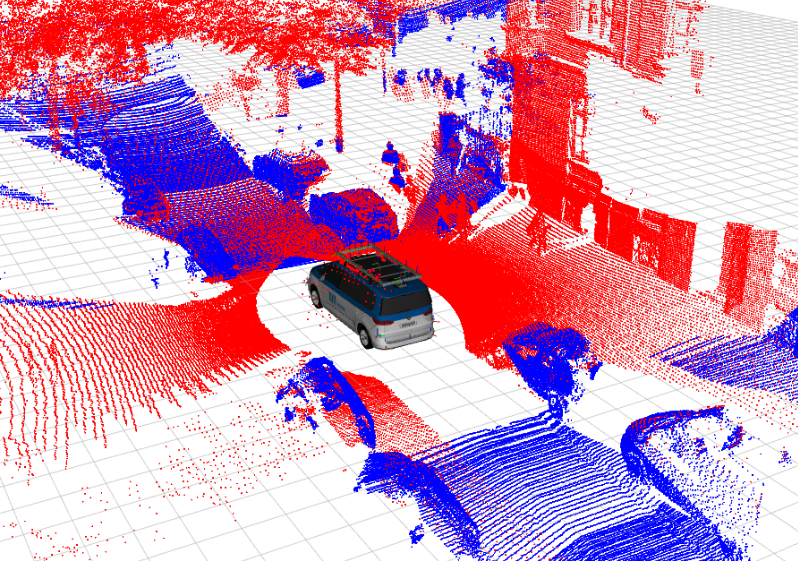
\includegraphics[width=\textwidth]{figures/edgar_3d.png}
  \end{minipage}\hfill
  \begin{minipage}{0.6\textwidth}
    \centering
    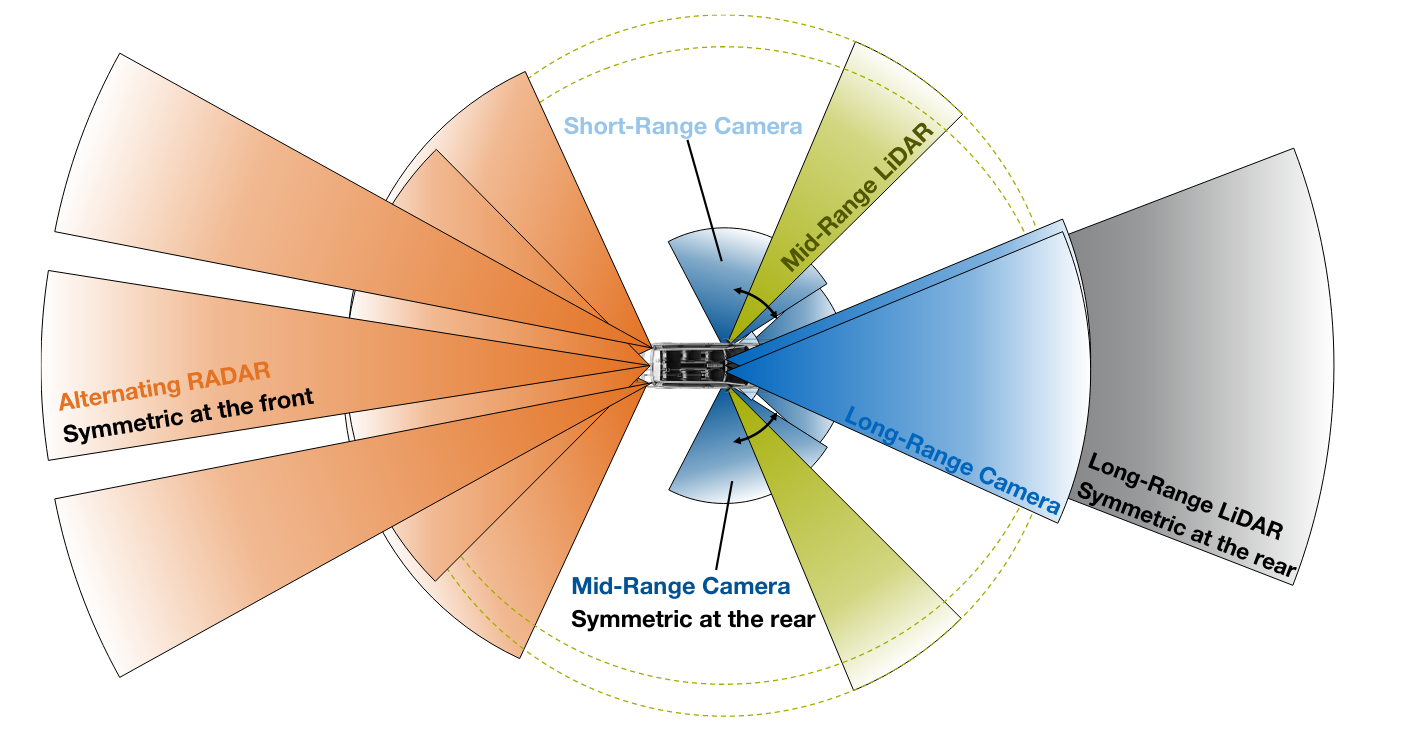
\includegraphics[width=\textwidth]{figures/edgar_sensors.png}
  \end{minipage}
  \caption{EDGAR Vehicle Sensors}
  \label{fig:edgar}%
\end{figure}%



\subsection{Previous Work in the FTM}

This project builds upon previous work conducted at the FTM in the field of environment perception 
for automated vehicles with 6D vision. Some of the key contributions include: 

\begin{enumerate}
  \item \textbf{Objektdetektion und Bewegungsprädiktion mittels eines Stereokamerasystems beim teleoperierten Fahren} \cite{previous_tfm_bauer}: Bauer 
  in his master's thesis developed a deterministic system for object detection based on the 6D vision of Daimler \cite{6d_vision_daimler}. The system 
  was implemented in C++ using the ADTF framework {Automotive Data and Time-Triggered Framework} and was capable of detecting and tracking objects in the vehicle's surroundings 
  with some real time limitations.

  \item \textbf{Weiterentwicklung und echtzeitfähige Umsetzung eines Stereo-Vision-basierten Bewegungsprädiktionssystems für die aktive Sicherheit von teleoperierten Fahrzeugen}
  Some time later in \cite{previous_tfm_gpu_implementation} Rotar continued Bauers work by implementing the system in GPU using CUDA to speed up the computationally intensive tasks.

  \item \textbf{Validation of an Obstacle Detection Approach for Teleoperation of Automated Vehicles:} Finally Pastor \cite{previous_tfm_pastor} started porting the system to ROS1
   to facilitate the integration with other modules in the EDGAR vehicle. The system was implemented without CUDA GPU acceleration
   and was not deployed in the EDGAR vehicle. The system also has some problem with the object detection.
\end{enumerate}

Building upon these previous contributions, this project aims to further improve deterministic perception by 
addressing key limitations found in prior implementations. 
In particular, this work will focus on enhancing computational efficiency, real-time feasibility, 
and system deployment within ROS2. These improvements will be detailed in the next section on objectives.